\documentclass[11pt,oneside]{article}

\usepackage[T1]{fontenc}
\usepackage[utf8]{inputenc}
\usepackage{amsmath}
\usepackage{sectsty}
\usepackage{tikz}
\usepackage[labelsep=period,font=small,labelfont=bf]{caption}
\usepackage[charter, cal = cmcal]{mathdesign}
\usepackage[scaled]{helvet}
\usepackage{pdflscape}
\usepackage{afterpage}
\usepackage[hyphens]{url}
\usepackage[colorlinks=true,citecolor=black]{hyperref}
\usepackage{booktabs}

% Highlighted notes
\usepackage{xcolor}
\usepackage{soul}
\newcommand{\note}[1]{\hl{[#1]}}

% Math commands
\DeclareMathOperator{\CVL}{CVL} % CV loss
\DeclareMathOperator{\CINC}{CINC} % CINC function
\DeclareMathOperator{\PRL}{PRL} % Proportional reduction in loss

% Section heading styling
\allsectionsfont{\sffamily}

% BibTeX
\usepackage{natbib}
\bibpunct{(}{)}{;}{a}{}{,}
\renewcommand{\harvardurl}[1]{\textbf{URL:} \url{#1}}

\title{
  Capability Ratios Predict Nothing%
  \thanks{%
    We thank Zach Jones and Marc Ratkovic for helpful discussions and advice.
    Bryan Rooney provided excellent research assistance.
    We also thank the authors listed in Table~\ref{tab:replications} for making their replication data publicly available.
    Replication code and a version history of the project are available at \url{https://github.com/brentonk/crpn}.
  }%
}
\author{%
  Robert J. Carroll%
  \thanks{%
    Assistant Professor, Department of Political Science, Florida State University.  Email:  \nolinkurl{RobCarrollFSU@gmail.com}.
  }%
  \and%
  Brenton Kenkel%
  \thanks{
    Assistant Professor, Department of Political Science, Vanderbilt University.
    Email: \nolinkurl{brenton.kenkel@vanderbilt.edu}.
  }%
}

\begin{document}

\maketitle

\begin{abstract}
  \noindent Modern approaches to political measurement have generally ignored the importance of out-of-sample predictive performance.
  This is problematic for two reasons: first, many of the abstractions scholars attempt to proxy for are themselves expectations; and second, the resulting measures are prone to overfitting.
  We advocate a data-driven approach to measurement focused on out-of-sample prediction.
  We demonstrate the effectiveness of the approach as it applies to proxying the expected outcome of militarized interstate disputes.
  The standard proxy for expected dispute outcomes, the ratio of material capability indices, has almost no predictive power.
  We use ensemble learning to construct a new measure from the same underlying covariates---the Dispute Outcome Expectations score, or DOE---whose predictive power far exceeds that of the standard measure.
  In replications of 18 empirical studies of international relations, we find that replacing standard capability measures with DOE scores usually improves both in-sample and out-of-sample goodness of fit.
\end{abstract}
\thispagestyle{empty}
\newpage
\setcounter{page}{1}


%!TEX root = doe.tex

Of all the great challenges in political science, perhaps none is more difficult than measuring theoretical quantities.
Most analysts care more about assessing relationships among variables rather than the quality with which a single variable is measured, and so many proceed by producing the simplest measure possible, often in the form of summated rating scales.\footnote{For a brief introduction, see \citet{spector2006}.}
The practice persists even though these simple measures often introduce \emph{ad hoc} assumptions that go untested, and authors are often apologetic for their use.
Happily, methodologists have resolved many old frustrations by developing better models for measuring a variety of quantities, from ideal points \citep{clinton2004} to judicial independence \citep{linzer2014} to democracy \citep{jackman2008}.
Meanwhile, scholars have amassed an impressive amount of data, particularly historical data.
Ideal points now use roll calls dating back to the American Constitutional Convention \citep{heckelman2013}; conflict scholars can access industrial output figures for each state dating back to the Napoleonic Wars \citep{singer1972}.
Improvements in computing power, coupled with scholarly ingenuity, ensure that this progress will continue for the forseeable future.

We should feel sanguine given these advances, but we should also pause to consider the nature of the measurement enterprise.
Our new data sets enable us to ask and answer meaningful measurement questions, and this often means doing more than taking unweighted averages of our new variables.
Put differently, when imposed on new and interesting data, crude measures seem especially crude---we cannot even complain that they are underfit, as they are not fit to data at all.
At the other extreme, measurement models with an abundance of parameters run the risk of overfitting:  the attribution of systematic importance to the random error inherent in any sample.
Likewise, as our data sets grow, we run the risk of attributing too much reliability (sociologically speaking) to our potentially overfit results.
Yet, to our knowledge, none of the recent advances in political measurement have taken out-of-sample performance into account; rather, attention is paid to developing and interpreting measures that best reflect extant data.\footnote{In contrast, structural modelers have paid increasing attention to overfitting problems\citep{pitt2002,preacher2006}, though most instruction retains the focus on fit.}

We aim to provide an approach to measurement that strikes a balance between the severely underfit and the potentially overfit.
In this article, we argue that proxies should be constructed to predict well and that measurement functions should be assessed accordingly.
We advocate a data-driven approach focused on out-of-sample prediction:  a proxy for the expectation of some political outcome ought to be a good predictor of that outcome.
When choosing among the variety of models available to construct a proxy variable, the data used to assess the model should not be the same as the data used to fit it.
Techniques that accomplish this division of labor through sample-splitting, such as cross-validation \citep{Efron:2012es}, should play a larger role in measurement construction.
We employ such techniques in developing a supervised measurement method that learns from the data---thus avoiding underfitting---while sidestepping overfitting problems.
Our arguments mirror those of \citet{Hill:2014ki}, who use cross-validation to assess the relative predictive power of many variables all thought to affect the same outcome.  Our focus, however, is on constructing measures rather than comparing them---in particular, we examine how to create proxies with the greatest ability to predict.

Though any measure suffers when a data set's unique peculiarities are assigned too much explanatory import, theoretical expectations provide special challenges.
To animate the situation (and to introduce our application to international conflict), imagine a real-world leader that must decide whether to start a war against another state.  Perhaps inspired by Santayana's observation that ``those who cannot remember the past are doomed to repeat it,'' the leader orders her statisticians to obtain data on the outcomes of previous conflicts and the material capabilities of their combatants.
The statisticians, of course, could use the data in a variety of ways, but the leader would care only that their results did the best job of predicting.
More to the point, the leader would care less that estimates of the relevant parameters fit the historical data as well as possible (as would be the case if the statisticans ran traditional logit or probit models alone) but instead would care more that the prediction was of high quality.
Indeed, to borrow another aphorism, we can reimagine the oft-lamented sin of ``fighting the last war'' \citep[e.g.][]{hart1972} as overfitting such historical models with excess weight placed on recent observations.
Yet, when we write down formal models of choice under uncertainty featuring actors like this leader, we operate on the assumption that that the expectation in question is, by definition, the predictor of the outcome---and, as such, is neither under- nor overfit to some other relevant data at the hypothetical decision-maker's disposal.

Like the leader, empirically-minded conflict scholars, especially those inspired by the bargaining model of war \citep{fearon1995}, often want good measures of outcome expectations.  
Consider the statistical model of power, status quo benefits, and militarized dispute onset analyzed by \citet{reed2008war}.
This model is especially relevant in that the authors aim to directly test a functional form result from the formal analysis provided by \citet{powell1996stability,powell1999}.
The question is as to how the effect of the distribution of capabilities, parameterized as $p$, on dispute onset varies with the distribution of status quo benefits, parameterized as $q$.
The authors take great pains to provide a good estimate of the latter; for the former, they rely on the previous literature, which has proceeded by estimating $p$ via \emph{a priori} transformations of existing indices of capability data.\footnote{The capability measures, Composite Indices of National Capabilities \citep{singer1972}, combine six variables covering states' industrial capacity, their population, and their wealth.}
Their resulting estimate ranges from 0 to 1---just as a probability does, highlighting the measure's theoretical roots as an expectation.
Indeed, \citet[Footnote 11, p. 1211]{reed2008war} note that $p$ captures ``the chances of prevailing in the costly lottery of war.''
They choose their preferred measure of $p$ because ``it is a simple description of the likelihood of either state's success in war,'' though whether this is more or less the case for any given measure is a question left unanswered.
On the other hand, the authors note that different measurement choices yield different substantive results in their ultimate regression of interest, highlighting the importance of the problem at hand.
Reed et al.'s approach is now quite standard; in a search of some of the top journals for empirical work in international relations,\footnote{These included the \emph{American Political Science Review}, \emph{American Journal of Political Science}, \emph{Journal of Politics}, \emph{International Organization}, and \emph{International Studies Quarterly}.} we found at least 94 articles published between 2005 and 2014 that construct similar proxies using the same data.
Since so many scholars care so deeply about dispute expectations, and since dispute expectations themselves provide so many measurement challenges, we believe our application to be relevant for theorists and empiricists alike.

Our results suggest that time spent doing right by the leader and the scholar is time well spent.  
We find that the typical CINC transformation---the capability ratio---fails to predict any dispute outcome other than the modal category of stalemate and barely improves out-of-sample predictive performance (0.8\%) over a null model.
Conversely, our method yields predictions with much more variation and improves out-of-sample predictive performance by 20\%.  This is especially noteworthy given that we use the same component variables from which the CINC score is constructed. 
This result is of major substantive interest:  a scholar armed only with the traditional measure and a logit routine would conclude that material capabilities have little effect on dispute outcomes, whereas our results suggest that material capabilities matter in a very real way.
More broadly, our results suggest that materiel remains an important component in a measure of power, which remains an especially murky concept in political science.
\citet[420]{singer1963inter} argues that ``power is to [political scientists] what money is to the economist,'' and in particular that ``power is a useful concept only in its relative sense;'' later, \citet[25]{singer1972} argued that relative power is ``not nearly as measurable'' as wealth.  
Our efforts, then, make a substantive contribution by advancing the discourse on the measurement of a key concept that has proven most elusive in the decades since these claims were first made.

We also find that the factors that influence victory in battle are not static and unchanging but rather have evolved over time.
We say this for two reasons.
First, in comparing pairs of models that include and omit time, models with time perform significantly better out-of-sample than models that do not include time.
This indicates that dispute outcomes have varied over time, but it does not imply that the effect of material components has.
However, we also find that many of the best-performing tree-based models feature time prominently in their resulting regression trees.
This \emph{does} suggest that other features' effects vary with time.
Though our results are sufficiently abstract that we cannot make strong claims about the nature of this evolution, we think this result is interesting enough to warrant further attention as scholars enhance our understanding of material power.

We also produce a new measure:  the Dispute Outcome Expectation, or DOE.
DOE scores retain the simple, probabilistic flavor advanced in Reed et al.'s description of the relationship between theory and data.
For every dyad-year (or directed-dyad year) covered by the Correlates of War data, we provide the probability that each state would win a hypothetical dispute and the probability of stalemate.
DOE scores therefore make intuitive sense when interpreted in plain language.
The DOE score also tends to work better in the kinds of regressions empirical conflict scholars care most about.
We replicated 18 recent empirical studies that utilized traditional measures and then replaced them with the DOE score.  
In 14 of them, the DOE score improved out-of-sample goodness of fit, and it improved in-sample fit 15 times.
In other words, in advocating for the DOE score, we are not asking applied scholars to give anything up at the bottom line.

The paper proceeds in five sections.
In the first, we argue for the importance of predictive power in constructing proxies and assessing measurement models' assumptions.
Section~\ref{sec:methods} describes the data and methods we use to construct a new proxy for expected dispute outcomes.
In Section~\ref{sec:scores}, we discuss the advantages and disadvantages of our new measure, the DOE score.
Section~\ref{sec:replications} provides the results of our replications.
The final section addresses next steps and concludes.

%%% Local Variables:
%%% mode: latex
%%% TeX-master: "doe"
%%% End:



\section{Predictive Power and Proxy Variables}

We are often interested in questions that link observed data to some unobserved quantity. 
This latter quantity may be unobserved because it is difficult (or impossible) to measure directly (like wealth) or because it is an abstraction (like the ideal point of a voter in a spatial model). 
In either case, the applied analyst faces a choice between omitting some potentially important variable and including some proxy variable in its stead \citep{stahlecker1993}. 
There is no best choice: some theoretical econometricians \citep[e.g.][]{mccallum1972} argue for the inclusion of all proxies (including crude ones), while others \citep[e.g.][]{maddala1977} support only the use of reliable proxies. 
Even those in the former camp, however, admit that reliable proxies perform better than unreliable ones.

Healthy disciplines utilize good measures for central concepts \citep{kuhn1977}, and so social science progresses, in part, by developing better ways to construct proxy variables.\footnote{Here we focus on the importance of models in producing measures; equal weight should be assigned to advances in the estimation of these models' relevant parameters, most notably to advances in Bayesian estimation \citep{jackman2001,martin2002,clinton2004,bafumi2005}.} 
Much recent progress is due to the development of measurement models.\footnote{Of course, the use of theory in the act of measurement is nothing new. 
  Economics retains its longstanding commitment to structural estimation whereby theory is used to uncover theoretically relevant quantities. 
  For current applications to the structural estimation of dynamic discrete-choice games (for example), see \citet{su2012} and \citet{egesdal2013}.} \citet[2]{jacoby2014} observes:
\begin{quote}
  ``All of us are comfortable with the notion of statistical \emph{models} that provide representations of structural relationships between variables.  But, modern social science also regards measurement as a model that pertains to each of the individual variables.  Careful attention and rigorous approaches are just as important for the latter type of models, as they are for the former.''
\end{quote}
Moreover, when the unobserved quantity is an abstraction, appropriate measurement models allow the analyst to perform direct tests that follow from the same set of assumptions as those used in the original, theoretical model. 
As \citet[355]{clinton2004} put it in the context of testing legislative behavior, ``it is inappropriate to use ideal points estimated under one set of assumptions (such as sincere voting over a unidimensional policy space) to test a different behavioral model (such as log-rolling).''

While better models (and better ways to estimate their parameters) have improved our measures of a variety of important quantities, it remains problematic that modern political measurement has ignored the importance of predictive power in producing proxies. 
This is odd, as seminal contributions to the literature utilize classification as a way to prove a new measure's superiority over extant ones. For example, in the classic paper on ideal point estimation in American legislatures, \citet[Table 3]{poole1985} report that a simple classification approach based on their NOMINATE scores correctly predicts over 80\% of legislative votes in most years in their data. Though their procedure estimates ideal points via the method of maximum likelihood rather than via a classification criterion, it remains that this analysis lies prone to textbook overfitting problems. 
In their analysis, Poole and Rosenthal estimate ideal points within a single Congressional session, and their classification analysis then uses those ideal points to assess voting within the same Congressional session. 
While many correct classifications reflect the spatial model's explanatory virtues, others may arise due to overfitting to the data within that Congressional session.

% TODO: This next paragraph is really good, and might merit being moved to the introduction, particularly as part of making clearer exactly what we're doing.

While ideal points may be of interest for purely explanatory purposes \citep{clarke2012}, many other quantities of interest are inherently forward-looking. 
For example, in the bargaining model of war \citep{fearon1995}, states' security decisions are largely a function of their expectations of winning a war.\footnote{Costs, too, play an important role, but their measurement is far more nuanced \citep{stiglitz2008,stiglitz2012}.} 
To animate the situation, imagine a real-world leader that must decide whether to start a war against another state. 
Perhaps inspired by Santayana's observation that ``those who cannot remember the past are condemned to repeat it,'' the leader orders her statisticians to obtain data on the outcomes of previous conflicts and the material capabilities of their combatants. 
The statisticians, of course, could use the data in a variety of ways to produce a prediction for the hypothetical war in question, but the leader would care only that the prediction was the one that did the best job of predicting. 
More to the point, the leader would care less that the relevant parameters fit the historical data as well as possible (as would be the case if the statisticians ran traditional logit or probit models alone) and would care more that the prediction was of high quality. 
Indeed, to borrow another aphorism, we can reimagine the oft-lamented sin of ``fighting the last war'' \citep[e.g.][]{hart1972} as overfitting such historical models with excess weight placed on recent observations. 
Just like the leader, users of the bargaining model want the estimate of war outcomes that predicts best rather than the one that fights the last war.

It is for these reasons that we advocate the train-validate-test approach common in machine learning. 
While orthodox approaches conform to maximization or minimization of relevant error or likelihood within the entire data set, we instead aim to optimize predictive performance.\footnote{Our formal criterion for predictive performance, the log loss function, is explicitly described in the methods section.} 
First, we split our data into a larger \emph{training set} used for model fitting and selection and a smaller \emph{test set} that we use to assess the predictive performance of our chosen model.
We then fit a variety of models to the training set in order to find the one with the best predictive performance.
At this point, if we were to pick the model that best fits the training data, we would likely end up with one that is overfit.
To prevent this, we assess model fit through cross-validation, which amounts to another layer of sample-splitting.
Finally, once we have chosen a model from the training set, we apply it to the test set to yield an accurate measure of its true predictive power when brought to previously unseen data.

This approach explicitly addresses the problems enumerated above: it avoids the overfitting problems associated with traditional measurement techniques and the model selection problems associated with attempts to bring new data to bear for predictive purposes. 
We believe that the costs of our approach---additional computation, interpretative nuance, and conservatism in inference---pale in comparison to these benefits. 

%%% Local Variables:
%%% mode: latex
%%% TeX-master: "doe"
%%% End:



\section{The Capability Ratio and Its Discontents}

Thanks in part to the popularity of formal models of choice under uncertainty, many unobserved quantities like those discussed above take the form of probabilities. 
Our application---expectations about war outcomes as parameterized by some probability $p \in [0,1]$---is no different.
We want to create a proxy for the chance that Country~A would prevail in a dispute against Country~B, given their observable characteristics, $x_A$ and $x_B$.
Since a measure of a probability must lie within the unit interval, a natural way to proceed is to propose an indexing function $g$, where $g(x) \geq 0$, and then take the ratio of indices,
\begin{equation}
  \label{eq:ratio}
  f(x_A, x_B)
  =
  \frac{g(x_A)}{g(x_A) + g(x_B)}.
\end{equation}
The quality of such a measure depends on both the selected characteristics and on the appropriateness of the indexing function~$g$.
This latter responsibility plays a large role in the development of good measures and is our primary area of focus.

Though simple, this enhanced ratio-based approach is remarkably powerful and finds use in a diverse array of applications. 
A classic success comes from the study of baseball outcomes, where the Pythagorean prediction \citep{james1983,miller2007} of a team's winning percentage is defined as
\begin{align*}
  f\left(\text{Runs Scored}, \text{Runs Allowed} ; \alpha\right) &= \frac{\text{Runs Scored}^\alpha}{\text{Runs Scored}^\alpha + \text{Runs Allowed}^\alpha},
\end{align*}
where $\alpha \geq 0$ adjusts $x$'s shape. 
Here the quest for the best-fitting $g$ amounts to estimating $\alpha$; \citet{james1983} originally proposed $\alpha = 2$ \emph{ad hoc}, and later analysts found that $\alpha = 1.83$ fit the data best. 
Though the analyses that produced this estimate suffer from the overfitting problems discussed above, the Pythagorean predictor still performs quite well when imposed upon out of sample data.

% TODO: Some of this notation collides with what we use for multiple imputation in the appendix.  Do we care?

When proxying for expected dispute outcomes, empirical conflict scholars normally use transformations of data on states' material capabilities. 
We now relate the typical transformation to our discussion of ratio-based measures above.
We begin by introducing some helpful notation: call the set of states $\mathcal{I} = \left\{1, \ldots, I\right\}$; the set of variables $\mathcal{J} = \left\{1,\ldots,J\right\}$; and the set of years $\mathcal{T} = \left\{1,\ldots, T\right\}$. 
Denote state $i$'s value for variable $j$ in time $t$ as $M_{ijt}$. 
The set of all data is $M$, and all data in year $t$ is $M_t$.
Define state $i$'s share of variable $j$ in year $t$ as
\begin{align*}
  S_{ijt}(M_{t}) &= \frac{M_{ijt}}{\sum_{\mathcal{I}} M_{ijt}}.
\end{align*}

We now introduce the \emph{CINC function}.\footnote{Here CINC stands for ``Composite Index of National Capability'' as given in the Correlates of War National Material Capabilities data \citep{singer1972}.} 
State $i$'s CINC score in year $t$ is its average share across all variables:
\begin{align*}
  \CINC_i(M_t) &= \frac{\sum_{\mathcal{J}} S_{ijt}}{\left|\mathcal{J}\right|}.
\end{align*}
State $i$'s CINC score therefore falls in $[0,1]$. 
The CINC score is the ``most commonly used measure'' of power in empirical conflict studies \citep[212]{kadera2004}.

Following the discussion in the previous section, the most intuitive CINC-based proxy for $p$ is a na\"{\i}ve \emph{capability ratio}:
\begin{align*}
  f_{\text{CR}}(M_t) &= \frac{\CINC_A(M_t)}{\CINC_A(M_t) + \CINC_B(M_t)}.
\end{align*}
Our approach, then, makes explicit the fact that $\CINC$ is simply a candidate $g$ function imposed upon annual material capability data $M_t$.

Many peculiarities emerge immediately. 
Two of these pertain to the CINC function itself. 
First, as has been documented, the CINC function is sensitive to changes in state membership over time \citep{organski1980,gleditsch1999,kadera2004}. 
Second, the CINC function's equal weighting of all indicators is entirely \emph{ad hoc}. 
For example, the CINC function assigns the same importance to military spending as it does to personal energy consumption. 
Whether this is an appropriate assignment is an empirical question that goes unanswered. 
Even on the tenuous assumption that $\CINC$ is a good data reduction technique on $M_t$, it is not clear whether it serves as a good $g$ function. 
Prior to entering $f_{\text{CR}}$, should the CINC scores be exponentiated given some parameter on returns to scale, or perhaps instead logged? 
Finally, even given that $\CINC$ is a useful index, we do not know whether a ratio-based approach is appropriate at all. 
In other words, taking the capability ratio at its word requires making a host of assumptions that may not hold well enough to make it useful in applications.\footnote{
  It is worth noting that some applications follow \citet{bremer1992} in using the explicit CINC ratio:
  \begin{align*}
    f_{\text{Bremer}}(M_t) &= \frac{\max\left\{\CINC_A(M_t),\CINC_B(M_t)\right\}}{\min\left\{\CINC_A(M_t),\CINC_B(M_t)\right\}}.
  \end{align*}
  Bremer's approach does not fall in $[0,1]$, though it could be transformed through a logit or probit CDF. 
  However, it is a monotonic transformation of the aforementioned capability ratio, and it suffers from similar problems anyway.
}

Yet it is widely used. Capability ratios (or similar manipulations of CINC scores) feature prominently in many recent empirical studies in international relations. 
As we might expect given the importance of the bargaining model, many of these \citep[e.g.][]{gartzke2007,salehyan2008} use capability ratios in regressions predicting the onset of a militarized interstate dispute. 
Still others focus on particular features of a militarized interstate dispute, such as the nature of its termination \citep{beardsley2008} or whether its combatants complied with laws of war \citep{morrow2007}. 
Still other studies focus on other phenomena not directly related to disputes, such as the onset of sanctions \citep{whang2013}, issue agreements \citep{mitchell2007}, or nuclear assistance provisions \citep{kroenig2009}. 
A more exhaustive survey of the use of capability ratios is beyond the scope of this paper, but suffice it to say that it is the go-to measure of relative power in international relations.

One might politely defend the capability ratio by noting that it asks the $\CINC$ function to perform a job it was not designed for. 
We would agree. 
It is worth noting, however, that early proponents of the $\CINC$ function \citep[24]{singer1972} sought to understand how ``uncertainty links[s] up with capability patterns on the one hand and with war or peace on the other.'' 
Writing over two decades before the classic introduction to the bargaining model of war \citep{fearon1995}, these authors lacked the abstract target---$p$---that we currently have, but their enterprise was largely similar. 
Though their focus on systemic, rather than dyadic, patterns reflects the dominant flavor of realism at the time, they still wanted to know how preponderance of power related to the decision to fight. 
So, while it remains true that the capability ratio is not meant to directly relate to $p$ in a bargaining model, the capability ratio was meant to tell us something about how uncertainly relates to war.

Remedying these problems by fitting a model---perhaps estimating an exponent on the CINC scores in $f_{\text{CR}}$, or weights for the CINC indicators---might be a laudable first step, but it would still suffer from functional form dependencies. 
The careful scholar might sidestep these by fitting an ensemble of models with different functional forms imposed, but so long as the ensemble is fit to the entire capability data set, it will suffer from overfitting and lose predictive power. 
In the next section, we outline our method for estimating $p$ that suffers neither from overfitting nor from pathologies in the $\CINC$-utilizing, ratio-based approach. 

%%% Local Variables:
%%% mode: latex
%%% TeX-master: "doe"
%%% End:



\section{Building a Better Proxy for Expected Dispute Outcomes}

\subsection{Data}

To evaluate the predictive performance of both the capability ratio and our alternative model, we use data on the outcomes of international disputes.
We combine the National Material Capabilities data \note{cite?} with information on the outcomes and participants of Militarized International Disputes between 1816 and 2007 \note{cite}.
Our data consist of $N = 1{,}740$ disputes, each between an ``initiator,'' or Country~A, and a ``target,'' or Country~B \note{footnote on this?}.
Every dispute outcome is either A~Wins, B~Wins, or Stalemate, which we denote by $Y_i \in \{A, B, \emptyset\}$, respectively.
In each dispute, we observe the year it took place, each disputant's raw material capability components, and each disputant's share of the system-wide total of each component at the time.\footnote{
  There are missing observations in the National Material Capabilities data.
  Consequently, about 17\% of the disputes we observe contain at least one missing cell.
  We use multiple imputation to deal with missingness \note{cite}; see the Appendix for details.
}
These predictors are collected in the vector $X_i$.

We want to measure the out-of-sample predictive power of various models, which means we cannot use the full dataset for model fitting.
Following common practice in machine learning, we randomly divide our sample into two parts: a \emph{training sample} for building and selecting models, and a \emph{test sample} for making out-of-sample predictions with a model built on the training sample \note{cite}.
We use an 80-20 split, resulting in a training sample of $N_{\text{train}} = 1{,}391$ disputes and a test sample of $N_{\text{test}} = 349$ disputes.\footnote{
  To avoid complications due to missing data, we draw the test sample exclusively from the subset of complete observations.
}
We exclusively use the training sample for all model tuning, fitting, and selection.
Even if we try to prevent overfitting in the training stage---which we do---we cannot rule out the possibility that the resulting model overfits the training data.
This is where the test sample comes in.
After selecting a model from the training data, we run the test sample through it to evaluate the model's out-of-sample predictive power.
As long as we do not use the test sample to make any further modeling decisions, this gives us an unbiased estimate of our chosen model's out-of-sample performance.

\subsection{Modeling Dispute Outcomes}

Our goal is to build the model that squeezes the most out-of-sample predictive power out of the few predictors available to us.\footnote{
  Having more predictors would, of course, be even better---we just want to see how much better we can do than the capability ratio without any additional data collection.
  Our method for constructing a measure would generalize easily to a setting with additional predictors.
}
To begin with, we must be a bit more specific about what we mean by ``predictive power.''
We define a \emph{model} as a function $f$ that maps from the predictor variables into the probability of each potential dispute outcome, $f(X_i) = (f_A(X_i), f_B(X_i), f_{\emptyset}(X_i))$.
Our metric for a model's predictive power is its \emph{log loss}, which is common in multinomial classification settings \note{cite?} and is closely related to the log-likelihood.
To calculate the log loss, we take a model's predicted probability of each observed outcome, take the average of their logged values, and multiply the resulting average by $-1$.
Smaller values of the log loss represent greater predictive accuracy, with a lower bound of~$0$ representing perfect prediction.\footnote{
  Predicted probabilities very close to~0 are trimmed to keep the log loss finite.
}
Formally, the log loss of a model~$f$ on the data $(X, Y)$ is
\begin{equation}
  \label{eq:log-loss}
  \ell(f, X, Y)
  =
  - \frac{1}{N} \sum_{i = 1}^{N} \sum_{t \in \{A, B, \emptyset\}}
  \mathbf{1} \{Y_i = t\} \log f_t(X_i).
\end{equation}

To select a model to use for out-of-sample prediction, we will fit a number of candidate models on the training data.
Since we cannot use the test data for model selection, this requires estimating each model's out-of-sample prediction error within the training sample.
We cannot rely on ordinary within-sample measures of fit (e.g., percent correctly predicted), as these will lead us to overfit to the training data.
Instead, we estimate each model's out-of-sample log loss via $K$-fold cross-validation \note{cite}.
We randomly assign each observation in the training sample to a ``fold'' $k \in \{1, \ldots, K\}$ and then fit each candidate model $K$ times, each time leaving one fold out of the fitting.\footnote{
  When fitting models with tuning parameters, we choose tuning parameters separately within each fold via another cross-validation loop, again using log loss as the objective function.
  In this case, when choosing the tuning parameters for the model fit to the full training data, we use different folds than those we use to estimate its out-of-fold log loss.
}
Assume that we have $M$ candidate models indexed by $m = 1, \ldots, M$, and let $\hat{f}_m^{(-k)}$ be the result when we fit the $m$'th candidate model to the data excluding fold~$k$.
Our estimate of the out-of-sample log loss of the $m$'th candidate model is its average out-of-fold log loss,
\begin{equation}
  \label{eq:cv-loss}
  \CVL(\hat{f}_m)
  =
  \frac{1}{K} \sum_{k=1}^K \ell \left(
    \hat{f}_m^{(-k)}, X^{(k)}, Y^{(k)}
  \right),
\end{equation}
where $(X^{(k)}, Y^{(k)})$ is the subset of training data assigned to fold~$k$.
Following usual practice, we use $K = 10$ cross-validation folds.

It is well known in the machine learning literature that averaging many models can lead to better predictive accuracy than using a single model \note{cite}.
Accordingly, instead of simply choosing the model with the lowest CV loss, we combine the models in a weighted average following the super learner algorithm \note{cite}.
Specifically, we select the weights $\hat{w}_1, \ldots, \hat{w}_M$ that solve
\begin{equation}
  \label{eq:super-learner}
  \begin{aligned}
    \min_{w_1, \ldots, w_M}
    &\quad
    \CVL \left(
      \sum_{m=1}^M w_m \hat{f}_m
    \right)
    \\
    \mbox{s.t.}
    &\quad
    w_1, \ldots, w_m \geq 0,
    \\
    &\quad
    w_1 + \ldots + w_m = 1,
  \end{aligned}
\end{equation}
where each $\hat{f}_m$ is the $m$'th candidate model fit to the full training data.
Our final model is the super learner, $\hat{f} = \sum_m \hat{w}_m \hat{f}_m$.
By definition, the CV loss of the super learner is no greater than that of the best candidate model.

To extract as much predictive power as possible from the material capability data, we examine a diverse array of candidate models to plug into the super learner.
Each candidate model must, of course, work with a categorical outcome variable and generate predicted probabilities.
Beyond that, we restrict our focus to classes of models that have been well studied in the machine learning or statistical literatures, settling on six: ordered logistic regression, $k$-nearest neighbors, random forests, neural networks, Gaussian processes, and support vector machines \note{cite each}.
We run each model on four sets of variables: the disputants' raw capability components and their capability component proportions, each with and without the year the dispute began.
We also include a null model (ordered logistic regression just on an intercept) and ordered logistic regression on the capability ratio, giving us $M = 26$ candidate models.

%%% Local Variables:
%%% mode: latex
%%% TeX-master: "oinc"
%%% End:



\section{The New Measure: Dispute Outcome Expectations}

We use the super learner results to construct a new proxy for expected dispute outcomes---one that predicts actual dispute outcomes much more accurately than the capability ratio does.
For any pair of countries at a particular point in time, whether or not they actually had a dispute with each other, we can use the super learner to ask, ``Based on what we know about their material capabilities, how would a dispute between these countries be likely to end?''
To construct the new proxy, we use the super learner to make predictions for every directed dyad--year in the international system between 1816 and 2007, the range of years covered by the National Material Capabilities data.
We call the resulting dataset the Dispute Outcome Expectations data, or DOE.
The DOE data contains predictions for more than 1.5~million directed dyad--years.\footnote{
  About 19~percent of directed dyad--years contain missing values of the capability components for at least one country.
  We average across imputations of the capabilities data to calculate the DOE scores for these cases.
  See the Appendix for details.
}

The DOE scores are naturally directed, since each dispute in our training data contains an initiating side and a target side.
However, many analyses in the international conflict literature (e.g., of dispute occurrence) use undirected data.
We calculate undirected DOE scores through a simple average of the directed values.
For example, to calculate the probability that the United States would win a dispute against the United Kingdom in 1816, we average its estimated chances of victory as an initiator (50~percent) and as a target (10~percent) to yield 30~percent.
If an analyst using the DOE data believed that the likely identity of an initiator in a hypothetical dispute were not a coin flip, she could take a different average of the directed scores to produce a more representative undirected score.

The DOE measures have two advantages over the capability ratio as a proxy for expected dispute outcomes.
First, they are direct measures of the quantity of primary interest to scholars of conflict: the probability that each state would win in a hypothetical dispute.
Although the capability ratio is a proportion, it cannot be interpreted as the probability of victory.
The ease of interpretation is particularly important for scholars who wish to control for expected dispute outcomes in a regression model.
The coefficient on a DOE score can be interpreted directly as the marginal effect of a state's chance of victory; the coefficient on the capability ratio cannot.
Second, as we have already seen, within the set of state pairs where disputes occur, the DOE measures are much better predictors of the outcome than the capability ratio is.
In short, they are superior proxies, and therefore are the appropriate choice for scholars who need an accurate measure of expected dispute outcomes.
The canonical correlation between the DOE scores and the capability ratio is 0.44 (for both the directed and undirected DOE scores), so the measures are related but distinct.

The DOE scores have one drawback worth mentioning: they should not be included as controls in regressions whose dependent variable is the outcome of a dispute or war.
This may seem contradictory, given how much effort we have just spent showing that DOE scores are superior predictors of dispute outcomes.
The reason they are superior is that, unlike the capability ratio, they are calibrated using real dispute data.
But this in turn means that DOE scores would be endogenous in a regression whose dependent variable is dispute outcomes---i.e., the same data we used to construct the DOE scores.
Another way to think about it is that the DOE score measures expectations of dispute outcomes, and there is no reason to think these expectations themselves have an independent effect on the outcomes.
So when we test causal hypotheses about dispute outcomes, we should control for raw capabilities, not expectations.
But when we are modeling dependent variables that might be affected by expectations, such as the onset of a crisis or a state's decision to join an ongoing conflict, we should use the best available proxy for those expectations---namely, the DOE scores.

\begin{figure}[tp]
  \centering
  \input{fig-vs}
  \vspace{-2em}
  \caption{
    Comparison of predicted outcome probabilities over time from the capability ratio and the super learner (DOE scores) for the United States versus Russia.
    These plots use the undirected scores.
  }
  \label{fig:vs}
\end{figure}

To illustrate the contrast between the capability ratio and DOE scores for forecasting hypothetical dispute outcomes, Figure~\ref{fig:vs} plot the two models' predictions over time for the United States versus Russia.
According to the capability ratio model, there was essentially no change between 1816 and 2007 in the likelihood of either side winning a dispute.
We need not dwell on the implausibility of this prediction.
Conversely, the DOE scores stack up with our intuitions relatively well: the predicted chance of a stalemate balloons during the Cold War, but the chance of victory by the United States picks up afterward.

In light of the DOE scores' superior predictive performance in the Militarized Interstate Disputes data, we are inclined to believe they dominate the capability ratio as a proxy for expected dispute outcomes.
Next, we test this conjecture by seeing if replacing the capability ratio with DOE scores in empirical models of international conflict improves their in-sample fit and out-of-sample predictive power.

%%% Local Variables:
%%% mode: latex
%%% TeX-master: "doe"
%%% End:



\section{Using the New Measure}
\label{sec:replications}

We have shown that our measure, the DOE score, predicts international dispute outcomes better than the current state of the art, the capability ratio.
But most recent studies of conflict do not aim to predict how disputes will end.
They focus on other dependent variables, and they usually only treat the capability ratio (or other functions of raw capabilities) as a control.
In this section, we investigate how well the DOE score performs as a replacement for the capability ratio in this more typical setting.
First, we replicate 18 recent empirical models of various international phenomena, finding that these models usually fit and predict better when we replace CINC-based measures with DOE scores.
After that, we provide some advice to practitioners on how to decide which measure---or measures---to include.

\subsection{Replication Analysis}

International relations scholars often control for the capability ratio as a proxy for expected outcomes when modeling dependent variables besides who wins, such as the onset or escalation of a dispute.
We have shown that the DOE score is a better proxy than the capability ratio, but it does not follow immediately that it is a better control variable in studies of conflict more generally.
Can we improve on these analyses---i.e., do our regressions fit the data better---if we replace the capability ratio with our new measure?
To address this question, we replicate 18 recent analyses of conflict using DOE scores in place of the capability ratio or other functions of CINC scores.
On the whole, we see that the models with DOE scores tend to have better in- and out-of-sample fit, though not always.

\afterpage{
  \clearpage
  \begin{landscape}
    \begin{table}[h]
      \centering
      \input{tab-replications}
      \caption{
        Summary of results from the replication analysis.
        In-sample goodness of fit is measured by the AIC and the \citet{Vuong:1989uf} test.
        Positive values of the Vuong test statistic indicate that the model with DOE terms fits better than the model with CINC terms, and vice versa for negative values.
        The Vuong test statistic has a standard normal distribution under the null hypothesis of no difference between the models, so values with a magnitude of $1.96$ or greater would lead us to reject the null hypothesis at the $0.05$ significance level.
        Out-of-sample fit is measured by proportional reduction in log loss relative to the null model, as reported in the last two columns.
        We use repeated 10-fold cross-validation to estimate each model's out-of-sample log loss, with 10 repetitions for models indicated by a dagger ($\dag$) and 100 repetitions for all others.
        The null model's log loss is estimated via leave-one-out cross-validation.
      }
      \label{tab:replications}
    \end{table}
  \end{landscape}
}

We constructed the set of replications by looking for empirical analyses of dyad-years (directed or undirected) that included the capability ratio or another function of CINC scores as a covariate.
Each study was published recently in a prominent political science or international relations journal.\footnote{%
  For details, see footnote~\ref{fn:replications}.
}
We examined only studies with publicly available replication data.
If we could not reproduce a study's main result or were unable to merge the DOE scores into the replication data (e.g., because of missing dyad-year identifiers), we excluded it from the analysis.
We also excluded studies that employed duration models or selection models, due to conceptual and technical problems with assessing their out-of-sample performance.
Lastly, we excluded studies in which our measure of expected dispute outcomes would be endogenous, namely those whose dependent variable was MID outcomes---the same data we used to construct the DOE scores---or a closely related quantity.
In the end, we were left with the 18 studies listed in Table~\ref{tab:replications}.

For each analysis in our sample, we begin by identifying the main statistical model reported in the paper, or at least a representative one.\footnote{%
  When no main model is apparent, our heuristic is to pick one on the log-likelihood--sample size frontier.
  Details of the model chosen from each paper and the functions of CINC and DOE scores used are in the Appendix.
}
We then estimate two models: the original model, and a replicated model where we replace any functions of CINC scores with their natural equivalents in DOE scores.
For example, if the capability ratio is logged in the original model, we log the DOE scores in the replicated model.
As a basic measure of each model's in-sample goodness of fit, we compute the \citet{Akaike:1974ih} Information Criterion,\footnote{%
  Because DOE scores are ternary, the replicated models typically have more parameters than their original counterparts.
  Hence we measure in-sample fit with the AIC, which penalizes over-parameterization, rather than the log-likelihood.
}
\begin{displaymath}
  \text{AIC}
  =
  2(\text{number of coefficients}) - 2(\text{log-likelihood}).
\end{displaymath}
The AIC is commonly used in model selection, with lower values representing better fit.
In addition, we compute the \citet{Vuong:1989uf} test of the null hypothesis that the original and replicated models fit equally well.\footnote{%
  We employ the standard Bayesian Information Criterion \citep{Schwarz:1978kh} correction to the Vuong test statistic.
}
To estimate each model's out-of-sample fit, we perform repeated 10-fold cross-validation.
Because each study has a discrete dependent variable, we again employ the log loss (equation~\eqref{eq:log-loss}) to measure out-of-sample fit.

Table~\ref{tab:replications} summarizes the results of the replication analysis.
In general, the models that include DOE scores do better than those with CINC scores by both in- and out-of-sample criteria.
Starting with in-sample fit, we see that the DOE model has a lower AIC than the CINC model in 15 of 18 cases.
Moreover, in more than half of those cases (8), under the Vuong test we would reject at the 0.05~significance level the null hypothesis that the models fit equally well.
The difference in fit is also statistically significant in all three cases where the CINC model has a lower AIC.
The results are similar for out-of-sample fit, with the DOE model having a greater proportional reduction in log loss in 14 cases.
The improvement due to using DOE scores is typically modest---about a single percentage point increase in the proportional reduction in log loss.
For context, keep in mind that these studies do not take capability measures as a key theoretical variable of interest.
In each regression, the capability measure is just one of a battery of control variables.
With so much else going on in these models, even a substantial improvement in the quality of the capability measure may lead to just a small increase in overall model fit or predictive power.

With such a small sample of replicated studies, we can only conjecture about why DOE performs better in some cases and worse in others.
We see that the cases where DOE is significantly better according to the Vuong test tend to have large sample sizes---but, then again, the study where it does worst has the largest $N$ in our sample.
In two of the replications where DOE performs worst, namely \citet{Bennett:2006gp} and \citet{Fordham:2008gs}, we see that both specifications include the raw CINC scores alongside or in lieu of the capability ratio.
These terms may be capturing monadic effects that the purely dyadic DOE scores miss.
On the other hand, in the other three analyses that include raw CINC scores \citep{Arena:2009gk,Zawahri:2011iy,Weeks:2012be}, the replication with DOE scores performs better by both AIC and cross-validation loss.

\subsection{Advice to Practitioners}

Seeing as neither the capability ratio nor DOE scores are uniformly better in typical applications, how should empirical scholars choose which one to include in their analysis?
Our main recommendation is a theory-driven approach.
When theory provides no guidance, we recommend either a data-driven approach or dropping capability measures altogether.

\begin{figure}[htp]
  \centering
  \input{dag-cap0-doe1}
  \caption{
    Raw capabilities only affect the outcome of interest through expectations.
  }
  \label{fig:dag-cap0-doe1}
\end{figure}

If theory suggests that material capabilities only affect the outcome of interest insofar as they shape expectations about how a dispute would end, then DOE scores are the best measure to control for.
Figure~\ref{fig:dag-cap0-doe1} contains a causal graph of this situation.
The clearest examples of theories where only expectations matter come from the formal literature on crisis bargaining.
Take \citeauthor{powell1999}'s~\citeyearpar{powell1999} theory of bargaining in the shadow of power.
War is possible only if the status quo distribution of benefits is far enough from the expected outcome of conflict that at least one state is dissatisfied.
An empirical model derived from this theory should control for DOE scores rather than the capability ratio or other poor proxies for expectations.

\begin{figure}[htp]
  \centering
  % Main document must include
% \usepackage{tikz}  % for the graphics
% \usepackage{etoolbox}  % for the if-then toggles

\providetoggle{cap-to-dv}
\providetoggle{doe-to-dv}

\toggletrue{cap-to-dv}
\toggletrue{doe-to-dv}

% Main document must include
% \usepackage{tikz}  % for the graphics
% \usepackage{etoolbox}  % for the if-then toggles

\providetoggle{cap-to-dv}
\providetoggle{doe-to-dv}

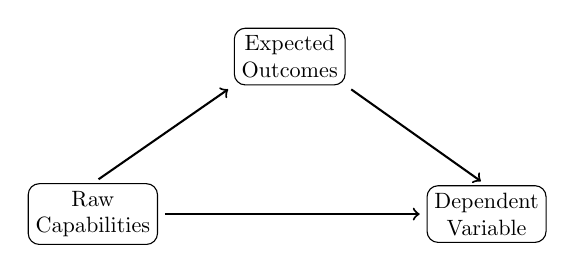
\begin{tikzpicture}[
  var/.style={
    rectangle,
    rounded corners,
    draw=black,
    align=center,
    scale=0.8
    }
  ]
  
  \node[var] (cap) at (0, 0) {Raw\\Capabilities};
  \node[var] (doe) at (2.5, 2) {Expected\\Outcomes};
  \node[var] (dv) at (5, 0) {Dependent\\Variable};

  \path[->, line width=0.75pt] (cap.north) edge[shorten <=0.25em, shorten >=0.25em] (doe.south west);
  \iftoggle{doe-to-dv}{\path[->, line width=0.75pt] (doe.south east) edge[shorten <=0.25em, shorten >=0.25em] (dv.north);}{}
  \iftoggle{cap-to-dv}{\path[->, line width=0.75pt] (cap.east) edge[shorten <=0.25em, shorten >=0.25em] (dv.west);}{}
\end{tikzpicture}

%%% Local Variables:
%%% mode: latex
%%% TeX-master: "doe"
%%% End:


  \caption{
    Raw capabilities affect the outcome of interest both directly and through expectations.
  }
  \label{fig:dag-cap1-doe1}
\end{figure}

If material capabilities affect the outcome both directly and indirectly via expectations, then it would be appropriate to control for both raw capabilities and expected dispute outcomes.
Figure~\ref{fig:dag-cap1-doe1} illustrates this scenario.
For example, imagine an empirical study of ``sinking costs'' via military mobilization in international crises \citep{fearon_signaling_1997}.
The initial movement of peaceful relations into a crisis, as well as early behavior at the bargaining table, might be shaped solely by states' expectations about dispute outcomes.
But if states build up their military as a way to signal resolve, independently of the effect on likely outcomes, then raw capabilities matter too.
When empirically modeling a theory like this, scholars should include both DOE scores and raw capability measures.
The ratio of CINC scores may or may not be the most appropriate way to capture raw capabilities---that, too, depends on the specifics of the theory.

\begin{figure}[htp]
  \centering
  % Main document must include
% \usepackage{tikz}  % for the graphics
% \usepackage{etoolbox}  % for the if-then toggles

\providetoggle{cap-to-dv}
\providetoggle{doe-to-dv}

\toggletrue{cap-to-dv}
\togglefalse{doe-to-dv}

% Main document must include
% \usepackage{tikz}  % for the graphics
% \usepackage{etoolbox}  % for the if-then toggles

\providetoggle{cap-to-dv}
\providetoggle{doe-to-dv}

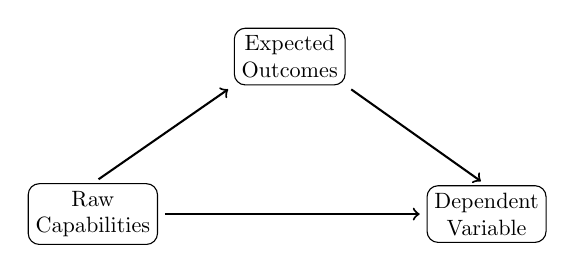
\begin{tikzpicture}[
  var/.style={
    rectangle,
    rounded corners,
    draw=black,
    align=center,
    scale=0.8
    }
  ]
  
  \node[var] (cap) at (0, 0) {Raw\\Capabilities};
  \node[var] (doe) at (2.5, 2) {Expected\\Outcomes};
  \node[var] (dv) at (5, 0) {Dependent\\Variable};

  \path[->, line width=0.75pt] (cap.north) edge[shorten <=0.25em, shorten >=0.25em] (doe.south west);
  \iftoggle{doe-to-dv}{\path[->, line width=0.75pt] (doe.south east) edge[shorten <=0.25em, shorten >=0.25em] (dv.north);}{}
  \iftoggle{cap-to-dv}{\path[->, line width=0.75pt] (cap.east) edge[shorten <=0.25em, shorten >=0.25em] (dv.west);}{}
\end{tikzpicture}

%%% Local Variables:
%%% mode: latex
%%% TeX-master: "doe"
%%% End:


  \caption{
    Raw capabilities directly affect the outcome of interest, but expectations do not.
  }
  \label{fig:dag-cap1-doe0}
\end{figure}

The last possibility to consider is that expectations do not affect the outcome of interest.
In this case, empirical models should only include raw capability measures, not DOE scores.
The clearest example is when the dispute outcome itself is the dependent variable.
First, absent some kind of self-fulfilling prophecy effect, we would expect actual capability holdings to drive outcomes more so than expectations.
Second, because DOE scores are calculated using the dispute outcome data, the DOE scores themselves are endogenous to observed outcomes, and thus should not be included as an independent variable when outcome is the dependent variable.\footnote{%
  In principle, this latter problem could be solved, albeit at great computational expense, by only using data for years up to $t-1$ to calculate the DOE score for year~$t$.
}

When there is no theory or the theory does not specify how material capabilities affect the outcome of interest, we recommend a data-driven approach.
The steps are the same ones we took in the replication analysis: determine a metric for model fit (whether in- or out-of-sample), run the model separately for each potential measure, and choose the best-fitting model.
Alternatively, if your theory says nothing about the relationship between capabilities and the outcome of interest, it may be best not to include capability measures at all.
A confounding variable, by definition, must be related to both the treatment and outcome of interest.
If raw capabilities are not supposed to affect the outcome either directly or through expectations, then they are not a confounder and there is no need to control for them.

%%% Local Variables:
%%% mode: latex
%%% TeX-master: "doe"
%%% End:



\section{Conclusion}
In this paper, we have argued that proxies should be constructed using predictive power as the criterion of interest, provided a method for doing so, and demonstrated the usefulness of the method in an application to measuring dispute outcomes.  We hope that our efforts will be of use both for both the DOE scores we provide and for the theoretical merits of our general argument.

In our application, the DOE scores outperform the extant proxy---the CINC-based capability ratio---in a number of important ways.  In pure terms, the DOE score more closely relates to what international relations care about:  the expected outcome of a dispute between two nations.  It therefore has a much more natural interpretation than the capability ratio.  It also lacks the \emph{ad hoc} assumptions imposed by both the CINC score and the ratio-based transformation used in most studies.  On the practical side, our replications suggest that the DOE score is a better contributor to the usual battery of variables included in the ever-expanding universe of international relations regressions.  We hope, then, that it will find use as scholars advance and test new claims.  

Though it represents a massive improvement over the \emph{status quo}, the DOE score could still be improved.  We have only included those variables that could be extracted from the data used to construct the capability ratio---namely, the six Correlates of War National Material Capabilities variables.  We did so consciously, as we wanted to demonstrate that our general approach could improve measures without introducing new covariates.  Having made our point, we look forward to seeing what the future holds for coming versions of DOE when new data is brought to bear on the problem.  At the risk of belaboring:  we created DOE using open-source software and have made our replication code available, and so anybody with a computer---and some patience!---could create a new version with new covariates.

On the theoretical side, we believe that our data-driven approach to measurement will prove useful for those wishing to proxy for other quantities.  All one needs is a set of predictor variables $\boldsymbol{x}$ and some outcome of interest $\boldsymbol{y}$---the $f$ we provide to map $\boldsymbol{x}$ to $\boldsymbol{y}$ will work.  Just as with introducing new covariates in any given application, future scholars can improve their proxies by including new models for evaluation in the super learner.  The general approach, however, remains unchanged.  Our application tasked us to create a proxy of a probabilistic expectation like those seen in formal models of choice under uncertainty, and similar applications provide a natural starting point for our method.  Doing so, however, requires good theory for just what it is that we hope to predict with our abstractions---for example, what outcome could we use variables related to democracy, like those used in the Polity score \citep{marshall2014}, to predict?  Hopefully readers from other subfields already have examples springing into their heads even as they read this sentence.  We ask them to turn their attention to these examples in the coming years.

We would like to conclude with a still broader point.  \citet{Breiman:2001fd} argues that statistical modelers fall into one of two cultures:  data modelers, who interpret models' estimates after assessing overall quality via in-sample goodness of fit; and algorithmic modelers, who seek algorithms that predict responses as well as possible given some set of covariates.\footnote{In case it is not obvious from our previous citations, Breiman self-identifies to the second culture.  He argues that 98\% of statisticians fall into the data modeling camp, which is a point we lack the expertise to assess.  However, we are comfortable saying that the vast majority of orthodox, empirical political scientists are data modelers.}  The method we advance is certainly algorithmic.  Our decision to adopt algorithmic modeling based on prediction, however, was not culture-driven---it was purpose-driven \citep{clarke2012}.  Most simply, many quantities to be proxied for are expectations, so they should be constructed with prediction in mind.  However, we realize that most political scientists remain, and will continue to remain, firmly entrenched in the data modeling culture.  Even now, in the middle of the identification revolution where analysts care more and more about the size of causal effects and less and less about traditional hypothesis testing, most empirically-minded political scientists---ourselves included---often find themselves interested in some hypothesis best assessed via data modeling.  This is why we took the DOE score's in- and out-of-sample performance in the replications so seriously:  despite its origins within the algorithmic culture, we want DOE to be of use to those who plan to remain in the data modeling culture.  Real people often reflect influences from seemingly contradictory cultures; we, as political scientists, are just as pleased that the DOE score performs better in regressions representative of our field as we are that it predicts better out out sample.  As new problems emerge and new solutions arise to solve them, we believe methodological pragmatism will be an important virtue.

Regardless of one's viewpoint, however, it remains that our discipline is measured in large part on the quality of its measures, and our approach has created at least one that performs better on a number of dimensions.

%%% Local Variables:
%%% mode: latex
%%% TeX-master: "doe"
%%% End:



\clearpage
\appendix
%!TEX root = doe.tex

\section{Appendix}

\subsection{National Material Capabilities Data}

Our predictors are taken from the National Material Capabilities (v4.0) dataset from the Correlates of War project \citepapp{singer1972}.\footnote{%
  Downloaded from \url{http://correlatesofwar.org/data-sets/national-material-capabilities/nmc-v4-data/at_download/file}.
}
The dataset contains observations on six variables for 14,199 country-years from 1816 to 2007.
For details on the variables and their measurement, see the NMC Codebook.\footnote{%
  Available at \url{http://correlatesofwar.org/data-sets/national-material-capabilities/nmc-codebook/at_download/file}.
}
Table~\ref{tab:summary} lists the proportions of zeroes and missing values among each variable.

\begin{table}[htp]
  \centering
  \input{tab-summary}
  \caption{
    Proportions of zeroes and missing values in each National Military Capability component variable.
  }
  \label{tab:summary}
\end{table}

All six variables are right-skewed.
Since five of the six variables are sometimes zero-valued (though all are non-negative), a logarithmic transformation is not appropriate.
Instead, to correct for skewness, we apply an inverse hyperbolic sine transformation \citepapp{Burbidge:1988gu} to each component:
\begin{equation}
  \label{eq:asinh}
  h(x, \theta)
  =
  \sinh^{-1} (\theta x)
  =
  \log \left(
    \theta x + \sqrt{(\theta x)^2 + 1}
  \right).
\end{equation}
We set the scale~$\theta$ separately for each component variable with the aim of making the transformed variable approximately normally distributed.
For each variable, we choose the value of $\theta \in \{2^d\}_{d=-10}^{10}$ that minimizes the Kolmogorov--Smirnov test statistic \citepapp{MasseyJr:2012jo} against a normal distribution with the same mean and variance.
Table~\ref{tab:summary} gives the scale selected for each component.
We use the transformed components in both the multiple imputation (see below) and the super learner training.

\subsection{Militarized Interstate Dispute Data}

Our sample and outcome variable are taken from the Militarized Interstate Disputes (v4.1) dataset from the Correlates of War project \citepapp{Palmer:2015hp}.\footnote{%
  Downloaded from \url{http://correlatesofwar.org/data-sets/MIDs/mid-level/at_download/file}.
}
The dataset records the participants and outcomes of interstate disputes from 1816 to 2010.
To avoid the problem of aggregating capabilities across multiple states, we exclude disputes with more than one state on either side.
We drop disputes that end in an outcome other than one side winning, one side yielding, or a stalemate;\footnote{%
  For details on other kinds of outcomes, see the MID Codebook.
}
we then collapse ``A Wins'' and ``B Yields'' into a single coding, and similarly for ``B Wins'' and ``A Yields.''
Finally, since the capabilities data only run through 2007, we exclude disputes that end after 2007.
In the end, we have $N = 1{,}740$ cases.

For each dispute in our dataset, we code the participating countries' capabilities using the values in the year the dispute began.
About 17~percent of disputes have at least one missing capability component for at least one participant.

\subsection{Multiple Imputation}

As noted above, all of the National Material Capabilities variables contain some missing values.
Following standard practice, we multiply impute the missing observations.
We perform the imputations via the \texttt{Amelia} software package \citepapp{pkg-Amelia}.

Rather than just impute the missing values in the final dataset of disputes, we impute the entire National Material Capabilities dataset.
This allows us to fully exploit the dataset's time-series cross-sectional structure in the imputation process \citepapp{honaker_what_2010}.
We include in the imputation model a cubic polynomial for time, interacted with country dummy variables.
As this results in an explosion in the number of parameters in the imputation model, we then impose a ridge prior equal to 0.1 percent of the observations in the dataset (see Section~4.7.1 of the \texttt{Amelia} package vignette).
We enforce the constraint that every imputed value be non-negative.
Finally, we impose an observation-level prior with mean zero and variance equal to that of the observed values of the corresponding component variable for every missing cell that meets the following criteria:
\begin{itemize}
  \item There are no non-zero observed values in the time series preceding the cell
  \item The first observed value that comes after the cell is zero
\end{itemize}
So, for example, if a country's urban population is zero from 1816 to 1840, missing from 1841 to 1849, and zero in 1850, we would impose this form of prior on the 1841--1849 values.
Diagnostic time series plots of observed versus imputed values within each data series, generated by the \texttt{tscsPlot()} function in \texttt{Amelia}, will be made available in the project's Dataverse.

The presence of missing data also complicates the calculations of country-by-country proportions of the total amount of each component by year.
One option is to recompute the annual totals in each imputed dataset, so that the resulting data will be logically consistent---in particular, all proportions will sum to one.
The drawback of this approach is that virtually every observation of the proportions will differ across the imputed datasets, even for countries with no missing data, since the annual totals will differ across imputations.
An alternative approach is to compute the annual totals using only the observed values.
The advantage is that non-missing observations will not vary across imputed datasets; the downside is that the proportions within each imputation will generally sum to more than one.
For our purposes in this paper, we think it is preferable to reduce variation across imputations, even at the expense of some internal consistency in the imputed datasets, so we take the latter approach: annual totals are the sums of only the observed values.

We impute $I = 10$ datasets of national capabilities according to the procedure laid out above, and we merge each with the training subset of our dispute data to yield $I$ training data imputations.
We run the super learner separately on each imputation, and our final model is an (unweighted) average of the $I$ super learners.

After training is complete, we run into missing data problems once again when calculating DOE scores.
To calculate predicted probabilities for dyads with missing values, we calculate a \emph{new} set of $I = 10$ imputations of the capabilities data and take an (unweighted) average of our model's predictions across the imputations.

\subsection{Super Learner Candidate Models}

We use the R statistical environment \citepapp{pkg-R} for all data analysis.
We fit, cross-validate, and calculate predictions from each candidate model through the \texttt{caret} package \citepapp{pkg-caret}.
We then construct the super learner by solving~\eqref{eq:super-learner} via base R's \texttt{constrOptim()} function for optimization with linear constraints.
Candidate models were drawn from \citet{Wu:2007ev} and \citet{FernandezDelgado:2014ul}.
Four of the algorithms named in \citet{Wu:2007ev}---$k$-means, Apriori, expectation maximization, and PageRank---are not suited for the prediction task at hand.
We also excluded AdaBoost due to long computation time and naive Bayes due to poor performance in initial tests.
Further details about each candidate model are summarized below.

\begin{itemize}
  \sloppy

  \item Ordered Logit \citepapp{McKelvey:2010gv}
  \begin{description}
    \item[Package] \texttt{MASS} \citepapp{pkg-MASS}
    \item[Tuning Parameters] None
    \item[Notes] In the ``Year'' models, the year of the dispute is included directly and interacted with each capability variable
  \end{description}

  \item C5.0 \citepapp{Quinlan:2015uc}
  \begin{description}
    \item[Package] \texttt{C50} \citepapp{pkg-c50}
    \item[Tuning Parameters] ~
    \begin{itemize}
      \item Number of boosting iterations (\texttt{trials}): selected via cross-validation from $\{1, 10, 20, 30, 40, 50\}$
      \item Whether to decompose the tree into a rule-based classifier (\texttt{model}): selected via cross-validation
      \item Whether to perform feature selection (\texttt{winnow}): selected via cross-validation
    \end{itemize}
  \end{description}

  \item Support Vector Machine \citepapp{Cortes:1995ie}
  \begin{description}
    \item[Package] \texttt{kernlab} \citepapp{pkg-kernlab}
    \item[Tuning Parameters] ~
    \begin{itemize}
      \item Kernel width (\texttt{sigma}): selected via cross-validation from $\{0.2, 0.4, 0.6, 0.8, 1\}$
      \item Constraint violation cost (\texttt{C}): selected via cross-validation from $\{\frac{1}{4}, \frac{1}{2}, 1, 2, 4\}$
    \end{itemize}
    \item[Notes] ~
    \begin{itemize}
      \item Radial basis kernel
      \item All predictors centered and scaled to have zero mean and unit variance
    \end{itemize}
  \end{description}

  \item $k$-Nearest Neighbors \citepapp{Cover:1967jq}
  \begin{description}
    \item[Package] \texttt{caret} \citepapp{pkg-caret}
    \item[Tuning Parameters] ~
    \begin{itemize}
      \item Number of nearest neighbors to average (\texttt{k}): selected via cross-validation from $\{25, 50, \ldots, 250\}$
    \end{itemize}
    \item[Notes] All predictors centered and scaled to have zero mean and unit variance
  \end{description}

  \item CART \citepapp{Breiman:1984tu}
  \begin{description}
    \item[Package] \texttt{rpart} \citepapp{pkg-rpart}
    \item[Tuning Parameters] ~
    \begin{itemize}
      \item Maximum tree depth (\texttt{maxdepth}): selected via cross-validation from $\{2, 3, \ldots, 9, 10\}$ (only up to 9 for models without year included)
    \end{itemize}
  \end{description}

  \item Random Forest \citepapp{Breiman:2001fb}
  \begin{description}
    \item[Package] \texttt{randomForest} \citepapp{pkg-randomForest}
    \item[Tuning Parameters] ~
    \begin{itemize}
      \item Number of predictors randomly sampled at each split (\texttt{mtry}): selected via cross-validation from $\{2, 4, \ldots, 12\}$
    \end{itemize}
    \item[Notes] 1,000 trees per fit
  \end{description}

  \item Averaged Neural Nets \citepapp{Ripley:1996vd}
  \begin{description}
    \item[Package] \texttt{nnet} \citepapp{pkg-MASS}, \texttt{caret} \citepapp{pkg-caret}
    \item[Tuning Parameters] ~
    \begin{itemize}
      \item Number of hidden layer units (\texttt{size}): selected via cross-validation from $\{1, 3, 5, 7, 9\}$
      \item Weight decay parameter (\texttt{decay}): selected via cross-validation from $\{10^0, 10^{-1}, 10^{-2}, 10^{-3}, 10^{-4}\}$
    \end{itemize}
    \item[Notes] Creates an ensemble of 10 neural nets, each initialized with different random number seeds
  \end{description}
\end{itemize}

\subsection{Replications}

\newcommand{\coef}[1]{\beta[\text{#1}]}

The following list contains basic information about each model in the replication study.
We carry out logistic and probit regressions via \texttt{glm()} in base R \citepapp{pkg-R}, multinomial logit via \texttt{multinom()} in the \texttt{nnet} package \citepapp{pkg-MASS}, ordered probit via \texttt{polr()} in the \texttt{MASS} package \citepapp{pkg-MASS}, and heteroskedastic probit via \texttt{hetglm()} in the \texttt{glmx} package \citepapp{pkg-glmx}.

\begin{table}[p]
  \centering
  \small
  \input{tab-replications-appendix}
  \caption{
    Full results of replication analyses.
    Cross-validation results are from repeated 10-fold cross-validation; those marked $\dag$ are repeated 10 times, all others 100 times.
  }
  \label{tab:replications-appendix}
\end{table}

\input{list-replications}


\bibliographystyleapp{apsr}
\bibliographyapp{doebib}

%%% Local Variables:
%%% mode: latex
%%% TeX-master: "doe"
%%% End:


\newpage
\bibliographystyle{apsr}
\bibliography{doebib}


\end{document}
